\subsubsection{Présentation du cas test}
    Pour tâcher d'observer la perte d'ordre des expériences numériques ont été menées grâce au logiciel Samurai.
    Les expériences ont portées sur la simulation de l'équation de diffusion en 1D avec une solution initiale 
    en forme de courbe de Gau\ss\, avec conditions de Dirichlet homogènes au bords. 
    Pour limiter les effets de bords (qui non pris en compte dans l'analyse précédente) le domaine à été pris \textit{grand}
    devant la largeur de la gaussienne initiale et le temps final assez petit pour que la diffusion n'atteigne pas le bord (qualitativement).
    L'erreur à été calculée comme la norme $L^2$ de l'erreur au temps final centrée sur la gaussienne
    \footnote{On calcul l'erreur autour de la gaussienne et pas sur tout le domaine car sinon elle serait artificiellement faible puisque la solution est quasi-nulle sur le reste du domaine qui a été pris grand pour éviter les effets de bord.}.
    Ce cas test est pertinent car il offre une solution lisse mais avec des gradients (donc l'AMR doit compresser à divers endroits)
    tout en offrant une solution analytique connue pour comparer l'erreur. 
    En effet le problème posé sur $\mathbb R^+ \times \mathbb R$ (sans conditions de bord): 
    \begin{align}
        \dt{u} &= \dxx{u},\label{eq:pb_dif}\\\notag
        u(t=0,x) &= \frac{1}{\sqrt{4 \pi a }} \exp\Bigl( - \frac{x^2}{4a}\Bigr).
    \end{align}
    Admet pour solution :
    \begin{align}
        u(t=0,x) = \frac{1}{\sqrt{4 \pi a (1+t)}} \exp\Bigl(-\frac{x^2}{4a(1+t)}\Bigr).
    \end{align}
    La solution numérique avec conditions de bord a été comparée avec la solution analytique sans conditions de bord, 
    au vu de la taille du domaine et des temps de simulation cela ne devrait pas interférer de manière mesurable.

    \begin{figure}[htbp]
        \centering
        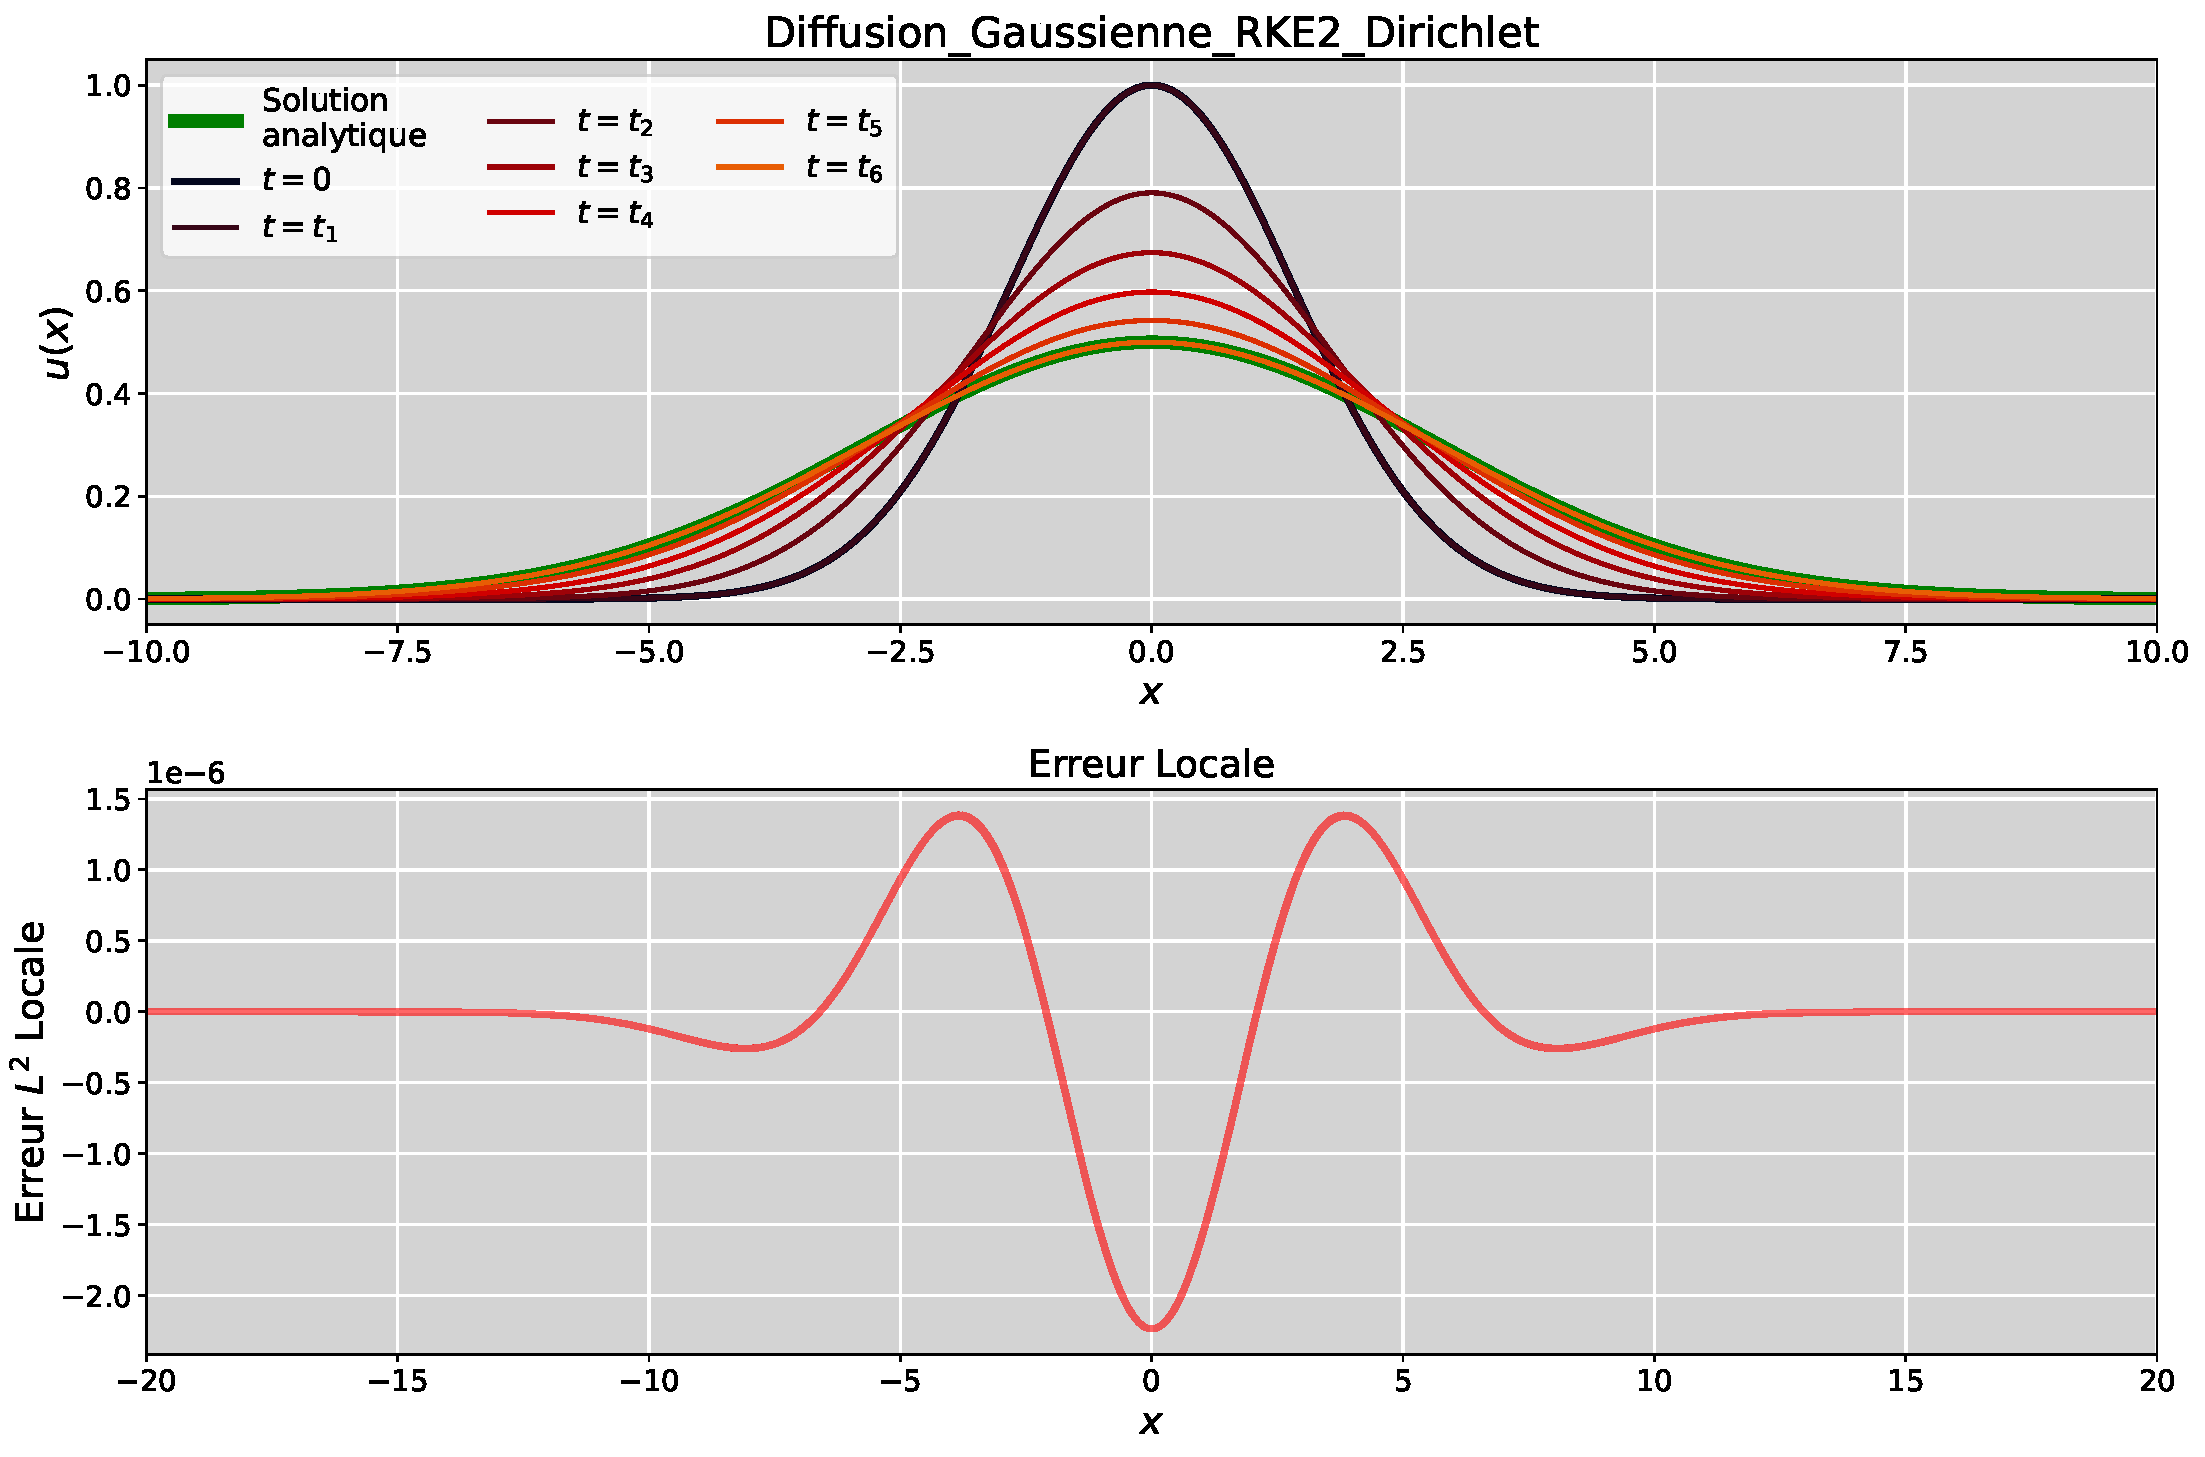
\includegraphics[width=.8\textwidth]{media/4_travail/1_AMR/illustration/Diffusion_Gaussienne_RKE2_Dirichlet.pdf}
        \caption{Illustration d'une simulation du cas test \ref{eq:pb_dif} avec conditions de Dirichlet homogène et
        affichage de l'erreur locale au temps final.}
        \label{fig:diffusion_gaussienne}
    \end{figure}
\subsubsection{Des défis expérimentaux}
    L'observation du mécanisme de perte d'ordre mis théoriquement à jour précédemment 
    est une tâche ardue.
    \paragraph{Une expérience exacte impossible à reproduire}
        Il n'est pas possible d'utiliser la méthode numérique utilisée dans l'étude théorique pour essayer de la valider expérimentalement. 
        En effet, la méthode est une RK2 explicite, elle impose sur ce problème de diffusion une condition de stabilité du type $\Delta t \propto \Delta x^2$,
        ce qui en pratique donne $\Delta t \ll \Delta x$. De fait, la majorité des erreurs sont liés au pas d'espace "grand" devant le pas de temps, et donc
        si l'on fixe le pas d'espace pour faire converger la méthode en temps, l'erreur est déjà saturée en temps et on n'observe rien. 
        C'est un classique de l'analyse numérique.
        \begin{figure}[htbp]
            \centering
            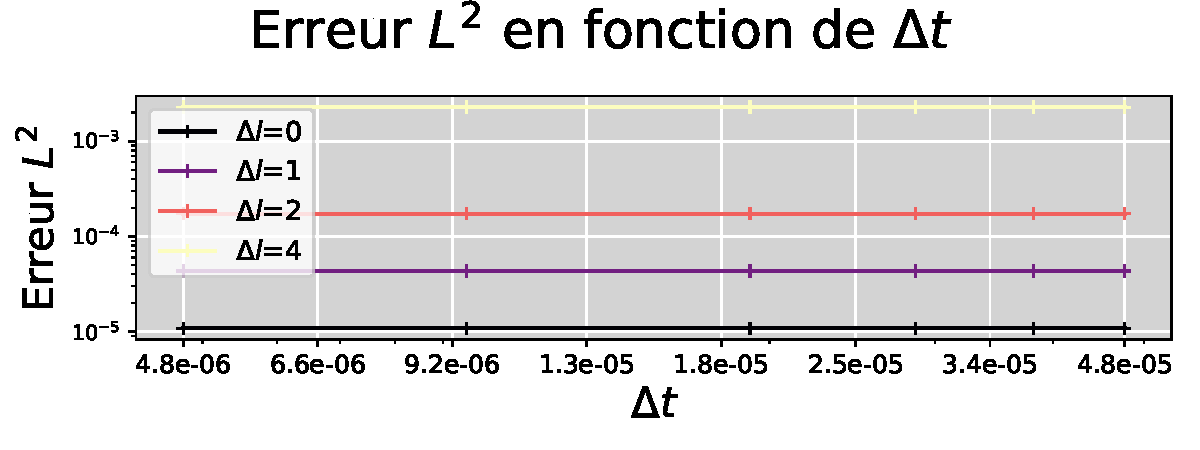
\includegraphics[width=\textwidth]{media/4_travail/1_AMR/convergence/convergence_temps_SATURATION.pdf}
            \caption{Saturation de la convergence temporelle avec une méthode RKE2 sur l'équation de diffusion. 
                        L'erreur L² stagne malgré la diminution du pas de temps, illustrant la domination 
                        de l'erreur spatiale due à la contrainte CFL $\Delta t \propto \Delta x^2$.}
            \label{fig:saturation_rke2}
        \end{figure}
    \paragraph{Une tentative infructueuse}
        Suite à cette limite, l'expérience a été retentée avec une méthode voisine, une RK2, mais sans contrainte de stabilité. 
        Le code de calcul Samurai a donc été relancé avec une méthode RK implicite d'ordre deux, plus précisément une SDIRK.
        Avec cette méthode, l'ordre deux est observé et ce qu'importe les paramètre de l'AMR.
        Plusieurs hypothèses peuvent expliquer ce résultat:
        \begin{enumerate}
            \item Le phénomène n'est pas présent sur cette méthode implicite.
            \item D'autres problèmes biaisent l'expérience (voir paragraphe suivant).
            \item Les calculs ou les prémisses du développement théorique précédent des équations équivalentes sont faux.
        \end{enumerate}
        \begin{figure}[htbp]
            \centering
            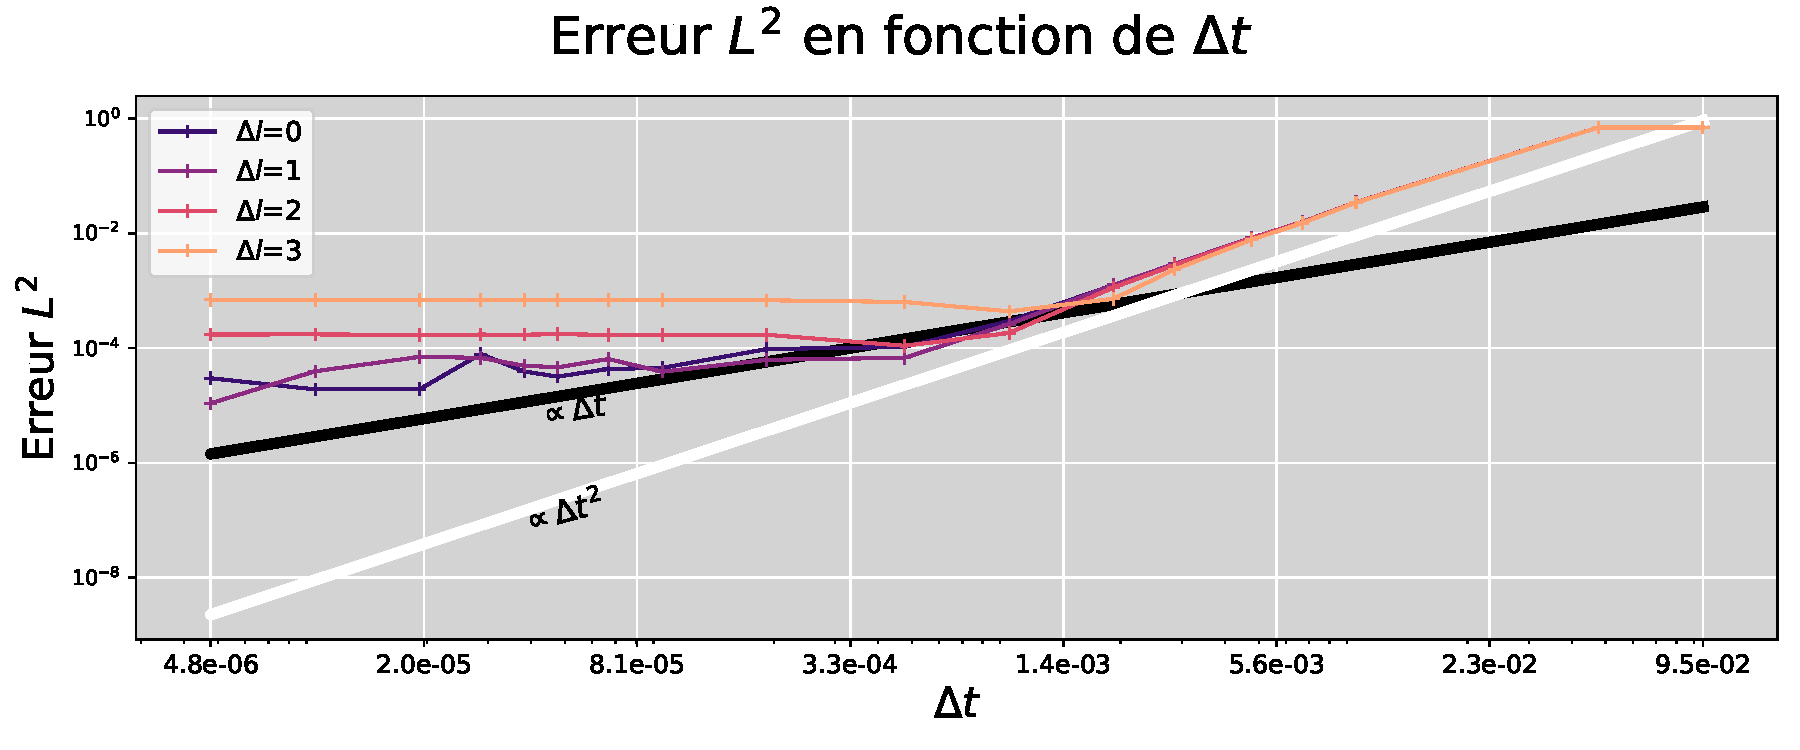
\includegraphics[width=\textwidth]{media/4_travail/1_AMR/convergence/convergence_temps_SDIRK_ORDRE2.pdf}
            \caption{Convergence temporelle d'ordre 2 avec une méthode SDIRK-RK2 sur l'équation de diffusion. 
                        L'ordre théorique est préservé indépendamment des paramètres MRA, contrastant avec 
                        nos prédictions théoriques établies pour les méthodes explicites.}
            \label{fig:convergence_sdirk}
        \end{figure}
    \paragraph{Des biais multiples}
        D'autres biais expérimentaux peuvent expliquer l'invisibilité du phénomène.
        Par exemple l'étude précédente ne prend pas en compte les conditions de bord.
        Une autre hypothèse est peut être que le maillage n'est compressé que localement 
        ce qui n'altère que peut être pas la convergence globale. 
        Enfin, dans les calculs théoriques précédents, il a été fait l'hypothèse que l'évaluation est faite au niveau le plus fin 
        (que la solution est entièrement reconstruite pour l'évaluation des flux), ce qui n'est pas fait en pratique. Cette idée viens du fait qu'intuitivement, 
        si l'on reconstruit jusqu'au niveau le plus fin les termes servant dans le calcul des flux, alors l'erreur devrait diminuer; c'est ce que suggère \cite{belloti_et_al_2025}.
        Cependant cette fonctionnalité n'étant pas encore disponible dans le logiciel de calcul, l'expérience a été réalisée sans reconstruire ls flux au niveau 
        le plus fin mais en prenant la valeur disponible au niveau courant de compression. Il semble peu probable que ce soit la cause de la non-observation du phénomène 
        de perte d'ordre mais cela reste un biais potentiel. Enfin peut être qu'un bug s'est glissé dans mon implémentation mais cela semble peu probable 
        puisque ce serait une erreur d'implémentation qu'il "améliore" l'ordre de convergence...
\subsubsection{... DEPEND DE LA SUITE ...}